%        File: illus_fig_utrecht_district.tex
%     Created: ven. févr. 28 08:00  2020 C
% Last Change: ven. févr. 28 08:00  2020 C
%
\documentclass{standalone}

\usepackage[utf8]{inputenc}
\usepackage{bm}
\usepackage{graphicx}
\usepackage{amsmath}
\usepackage{amssymb}
%\usepackage[normalem]{ulem}
\usepackage{dsfont}
\usepackage{mathtools}
\usepackage{graphics}
\usepackage{hyperref}
\usepackage{subfig}
\usepackage{tikz}
%\usepackage{lineno}
%\usepackage{xr}
\usepackage{subfig}
\begin{document}
\begin{tabular}[h]{cccc}
				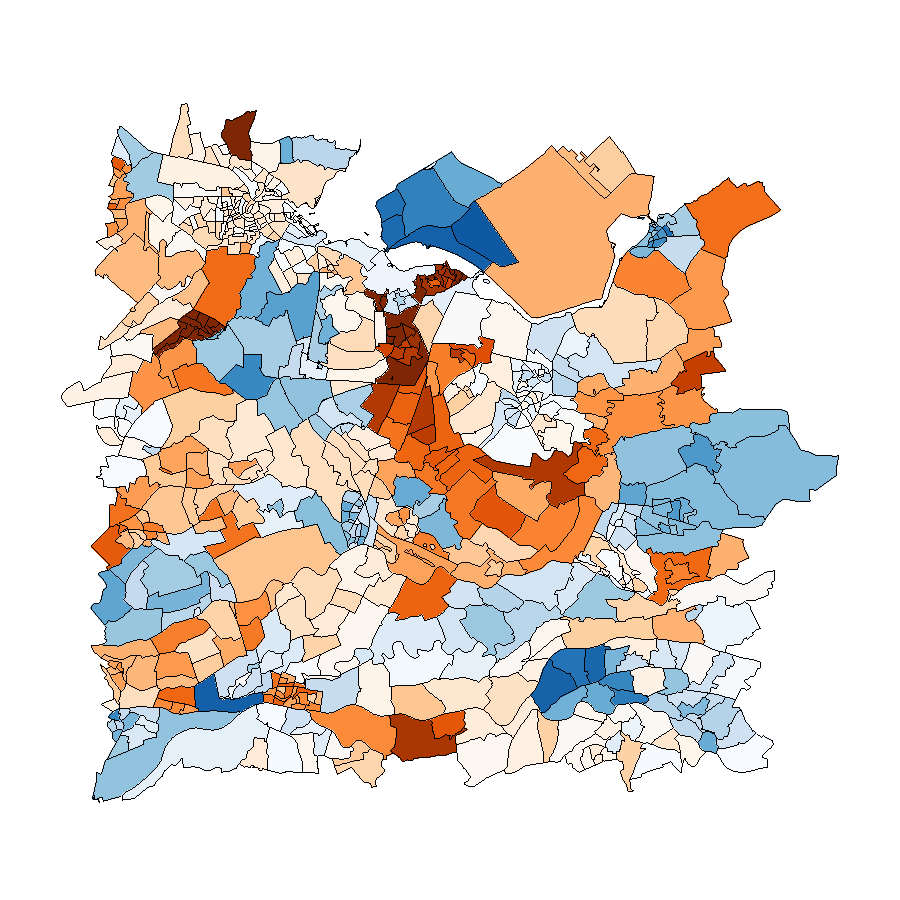
\includegraphics[width = 7cm, keepaspectratio]{../figure/graphical_abstract/graphical_abstract_utrecht_district1.pdf} &
				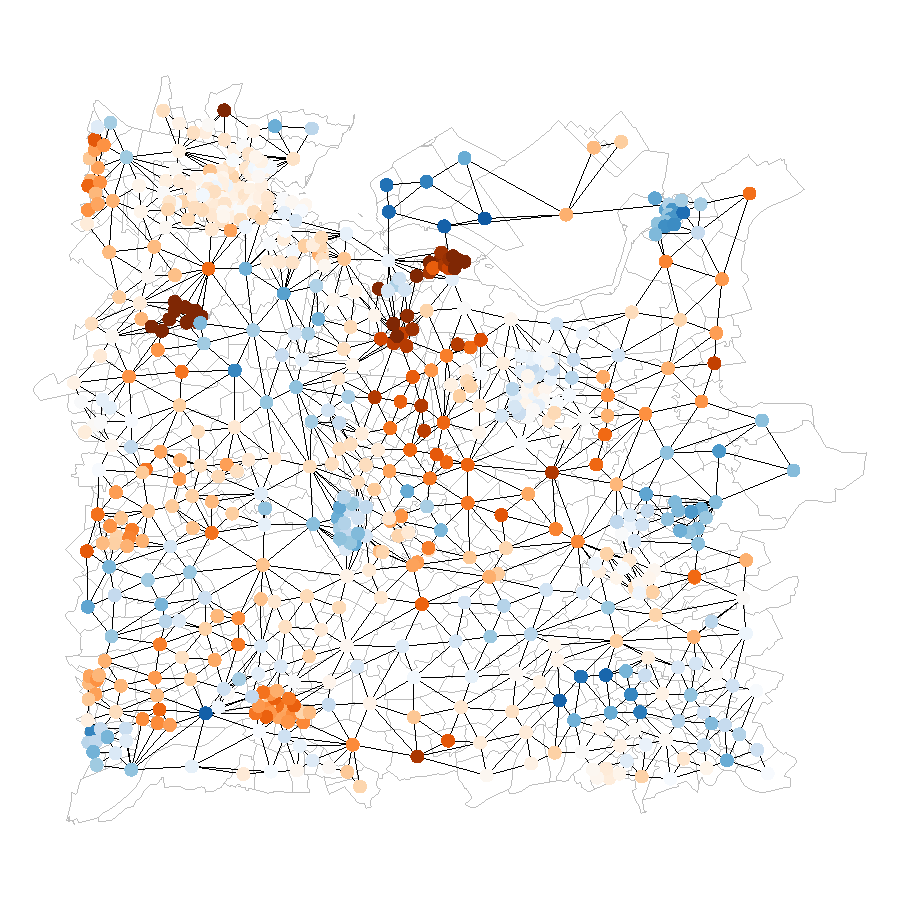
\includegraphics[width = 7cm, keepaspectratio]{../figure/graphical_abstract/graphical_abstract_utrecht_district2.pdf}  \vspace{-0.5cm}\\
				1. Noisy spatial signal & 2. Adding adjacency graph \\
				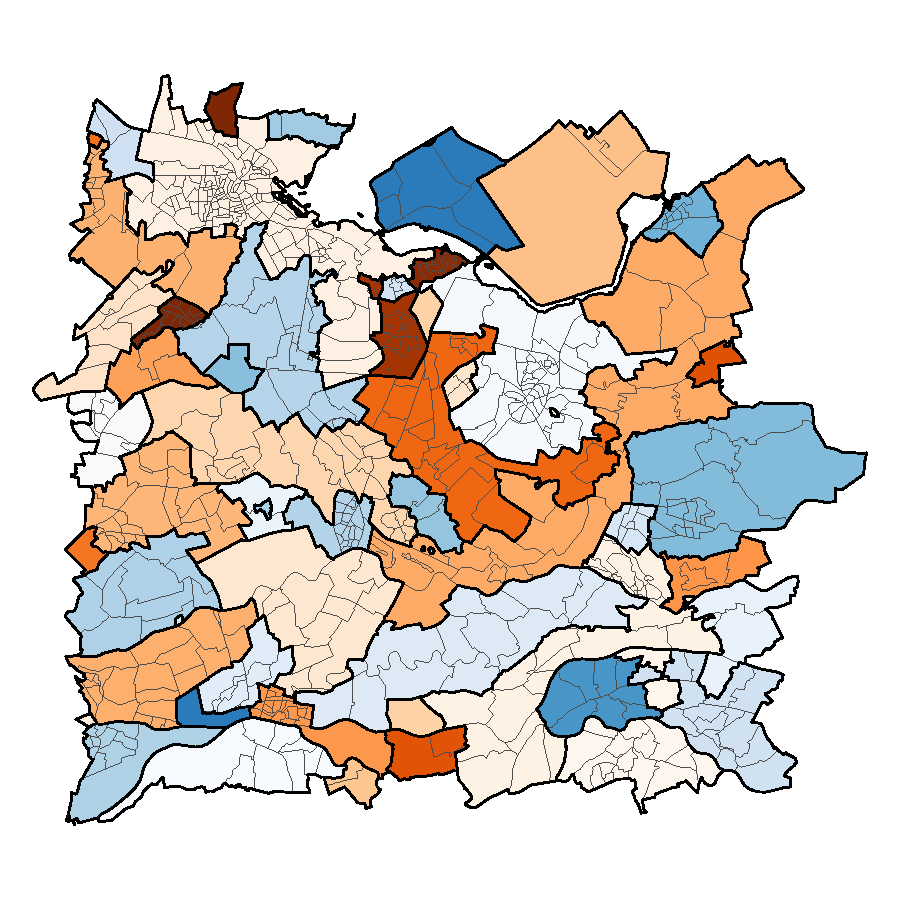
\includegraphics[width = 7cm, keepaspectratio]{../figure/graphical_abstract/graphical_abstract_utrecht_district3.pdf} &
				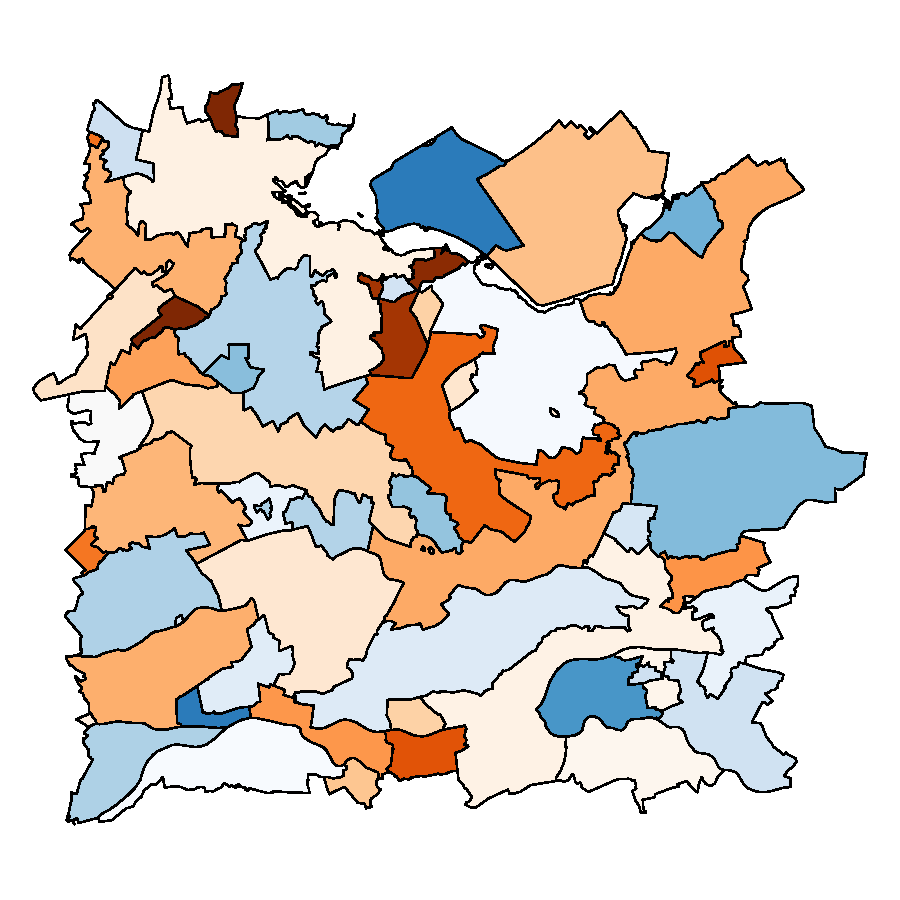
\includegraphics[width = 7cm, keepaspectratio]{../figure/graphical_abstract/graphical_abstract_utrecht_district4.pdf} \vspace{-0.5cm}\\
				3. Estimated piecewise-constant signal & 4. Highlighting zones of equal value
\end{tabular}
%\begin{figure}
		%\centering
		%\subfloat[]{
				%\includegraphics[width = 0.45\textwidth]{illus_fig_utrecht1.pdf}
		%}
		%\hfil
		%\subfloat[]{
				%\includegraphics[width = 0.45\textwidth]{illus_fig_utrecht2.pdf}
		%}
		%\hfil
		%\subfloat[]{
				%\includegraphics[width = 0.45\textwidth]{illus_fig_utrecht3.pdf}
		%}
		%\hfil
		%\subfloat[]{
				%\includegraphics[width = 0.45\textwidth]{illus_fig_utrecht4.pdf}
		%}
		%\caption{}
		%\label{fig:}
%\end{figure}
\end{document}


